\documentclass[11pt,a4paper]{article}
\usepackage{epsfig,colordvi,latexsym}
\usepackage{amsmath}
\usepackage{amsfonts}
\usepackage{amssymb}
\usepackage{graphicx}
\usepackage{color}
\usepackage{tikz}  %  for VMCON flowchart in Appendix A
\usepackage{url}
\usepackage{hyperref}
\usepackage{framed}
\usetikzlibrary{trees}



\pretolerance=10000
\topmargin=0mm
\headheight=0mm
\headsep=8mm
\textwidth=170mm
\textheight=240mm
\footskip=10mm
\oddsidemargin=0mm
\evensidemargin=-12mm
\parskip=2mm
\parindent=0mm


\setcounter{secnumdepth}{3}
\newcommand{\indat}{\mbox{\texttt{IN.DAT}}}
\newcommand{\mfile}{\mbox{\texttt{MFILE.DAT}}}
\newcommand{\outdat}{\mbox{\texttt{OUT.DAT}}}
\newcommand{\plotdat}{\mbox{\texttt{PLOT.DAT}}}
\newcommand{\process}{\mbox{\texttt{PROCESS}}}
\newcommand{\vmcon}{\mbox{\texttt{VMCON}}}
\renewcommand{\vec}[1]{\boldsymbol{#1}}

%%%%%%%%%%%%%%%%%%%%%%%%%%%%%%%%%%%%%%%%%%%%%%%
% Add here the date of the latest change and the code revision number
\newcommand{\version}{
15 July 2019
\hfill
PROCESS version: 1.0.16
}
%%%%%%%%%%%%%%%%%%%%%%%%%%%%%%%%%%%%%%%%%%%%%%%

\newcommand{\setheader}[1]
 {\markright{\rlap{\lower0.8ex\hbox to\textwidth{\hrulefill}}{\bf#1}}}
\newcommand{\mychapter}[1]{\small\normalsize
 \setcounter{footnote}{0}
 \chapter{#1}
 \pagestyle{myheadings}
 \setheader{Chapter \thechapter\hspace{0.8em}#1}}
\newcommand{\myappendix}[1]{\small\normalsize
 \setcounter{footnote}{0}
 \chapter{#1}
 \pagestyle{myheadings}
 \setheader{Appendix \thechapter\hspace{0.8em}#1}}

\begin{document}

\footnotesize
\hfill

\vspace*{4cm}
\begin{center}
\Huge The VMCON optimisation solver explained\\
~\\ \LARGE The PROCESS team: P.\ J.\ Knight, M.\ D.\ Kovari, H.\ Lux, J.\ Morris\\
~\\ \Large Culham Centre for Fusion Energy/ United Kingdom Atomic Energy Authority\\
Culham Science Centre, Abingdon, Oxon, OX14 3DB, UK
\end{center}
\normalsize
To give the user a better understanding of the optimisation solver implemented
in \process\/ and the interpretation of its results, we give a short
introduction into the mathematical background for solving these type of
problems as well as the specific algorithm used.

In section \ref{sec:GNPP}, the general nonlinear programming problem is
defined, which is the mathematical description of our problem. This problem is
typically formulated using Lagrange multipliers (c.f. \ref{sec:Lagrange}) and
is solved numerically most efficiently using sequential quadratic programming
(c.f. \ref{sec:SQP}). The Fortran subroutine that is used to implement such an
optimisation solver in \process\/ is called \vmcon\ (c.f. \ref{sec:vmcon}),
which iterates between solving a local quadratic subproblem
(c.f. \ref{sec:QSP}) and a one dimensional line search
(c.f. \ref{sec:linesearch}). As the method uses a quasi-Newtonian approach the
Hessian matrix is approximated by a variant of the
Broyden-Fletcher-Goldfarb-Shanno update (\ref{sec:BFGS}). Section
\ref{sec:symbols} summarises the symbol convention used in this chapter.

\vfill
\footnotesize
\version
\normalsize
\newpage


\newcommand{\ifail}{\mbox{\texttt{ifail}}}
\newcommand{\mat}[1]{\mathbf{#1}}

%%%%%%%%%%%%%%%%%%%%%%%%%%%%%%%%%%%%%%
%for tikz flow chart 
%%%%%%%%%%%%%%%%%%%%%%%%%%%%%%%%%%%%%%
\usetikzlibrary{arrows}
% Define the layers to draw the diagram
\pgfdeclarelayer{background}
\pgfsetlayers{background,main}

% Define block styles  
\tikzstyle{boxes} = [draw, fill=blue!20, text centered,
   text width=8em, minimum width=10em, minimum height=3em, rounded corners]
\tikzstyle{texto} = [above, text width=8em, text centered]
\tikzstyle{linepart} = [draw, thick, color=black!50, -latex', dashed]
\tikzstyle{line} = [draw, thick, color=black!50, -latex']
\tikzstyle{urred}=[draw, text centered, minimum height=0.01em,fill=red!20]
\tikzstyle{urgreen}=[draw, text centered, minimum height=0.01em, fill=green!20]

\tikzstyle{every node}=[]
\tikzstyle{selected}=[]
\tikzstyle{optional}=[]
 
\newcommand{\boxes}[2]{node (p#1) [boxes] {#2}}
\newcommand{\boxwsubs}[3]{node(p#1) [boxes]{#2:  {\scriptsize \begin{itemize}\item #3 \end{itemize}}}}

% Draw background
\newcommand{\mybackground}[5]{%
  \begin{pgfonlayer}{background}
    % Left-top corner of the background rectangle
    \path (#1.west |- #2.north)+(-0.5,0.5) node (a1) {};
    % Right-bottom corner of the background rectanle
    \path (#3.east |- #4.south)+(+0.5,-0.25) node (a2) {};
    % Draw the background
    \path[fill=yellow!20,rounded corners, draw=black!50, dashed]
      (a1) rectangle (a2);
    \path (a1.east |- a1.south)+(0.8,-0.3) node (u1)[texto]
          {\scriptsize{\bf #5}};
  \end{pgfonlayer}}

\newcommand{\outerbackground}[5]{%
  \begin{pgfonlayer}{background}
    % Left-top corner of the background rectangle
    \path (#1.west |- #2.north)+(-2.0,0.5) node (a1) {};
    % Right-bottom corner of the background rectanle
    \path (#3.east |- #4.south)+(+1.0,-0.5) node (a2) {};
    % Draw the background
    \path[fill=white!20,rounded corners, draw=black!50, dashed]
      (a1) rectangle (a2);
    \path (a1.east |- a1.south)+(1.3,-0.5) node (u1)[texto]
          { {\bf #5}};
  \end{pgfonlayer}}

\newcommand{\exit}[2]{%
  \path (#1.east)+(+5.0,0.0) node (urtmp)[urred] {\texttt{ifail} = #2};
  \path [line] (#1.east) -- node [above]
    {} (urtmp);}

\newcommand{\exitsucc}[2]{%
  \path (#1.east)+(+5.0,0.0) node (urtmp)[urgreen] {\texttt{ifail} = #2};
  \path [line] (#1.east) -- node [above]
    {} (urtmp);}

\newcommand{\exitleft}[2]{%
  \path (#1.east)+(+7.5,0.0) node (urtmp)[urred] {\texttt{ifail} = #2};
  \path [line] (#1.east) -- node [above]
    {} (urtmp);}

\newcommand{\exitright}[2]{%
  \path (#1.east)+(+2.5,0.0) node (urtmp)[urred] {\texttt{ifail} = #2};
  \path [line] (#1.east) -- node [above]
    {} (urtmp);}

\newcommand{\exitlower}[2]{%
  \path (#1.east)+(+5.,-0.25) node (urtmp)[urred] {\texttt{ifail} = #2};
  \path [line] (#1.east)+(0.0,-0.25) -- node [above]
    {} (urtmp);}

\newcommand{\exithigher}[2]{%
  \path (#1.east)+(+5.,0.25) node (urtmp)[urred] {i\texttt{fail} = #2};
  \path [line] (#1.east)+(0.0,0.25) -- node [above]
    {} (urtmp);}


\label{app:Opt}




\section{The General Nonlinear Programming Problem}
\label{sec:GNPP}
Mathematically the {\it general nonlinear programming problem} or {\it
  nonlinear constrained optimisation problem} is defined as
\begin{subequations}
\label{eqn:NPP}
\begin{align}
\textnormal{minimise } f(\vec{x}), & \\
\textnormal{subject to } c_i(\vec{x}) &= 0, & i&=1,\dots,k,\\
\label{eqn:NPP3}
\textnormal{and } c_i(\vec{x}) &\geq 0, & i&=k+1,\dots,m,
\end{align}
\end{subequations}
where both the {\it objective function}\footnote{Please note that what is
  called {\it figure of merit} in \process\/ is called {\it objective
    function} in the mathematical optimisation context. Hence, both names are
  used equivalently in this document.} $f(\vec{x})$ and the {\it constraints}
$c_i(\vec{x})$ are nonlinear functions of the $n$-dimensional vector of
variables $\vec{x}$ with bounds $\vec{x} \in \Omega$. In this context, all
$\vec{x}\in\Omega$ that fulfill the constraints $c_i(\vec{x})$ are called {\it
  feasible}. They describe the allowed space in which we are trying to
optimise the objective function $f(\vec{x})$. Note that any maximisation
problem can be written as a minimisation by using
$f_{\mbox{\scriptsize{new}}}(\vec{x}) = - f(\vec{x})$ and that any equality
constraint $c(\vec{x}) = a$ can be rewritten as
$c_{\mbox{\scriptsize{new}}}(\vec{x}) = c(\vec{x}) - a = 0$. Any inequality
constraint can therefore be rearranged analogously to fit the form described
in eq. \ref{eqn:NPP3}.

\section{The Lagrange Method}
\label{sec:Lagrange}

\begin{figure}[tbph]
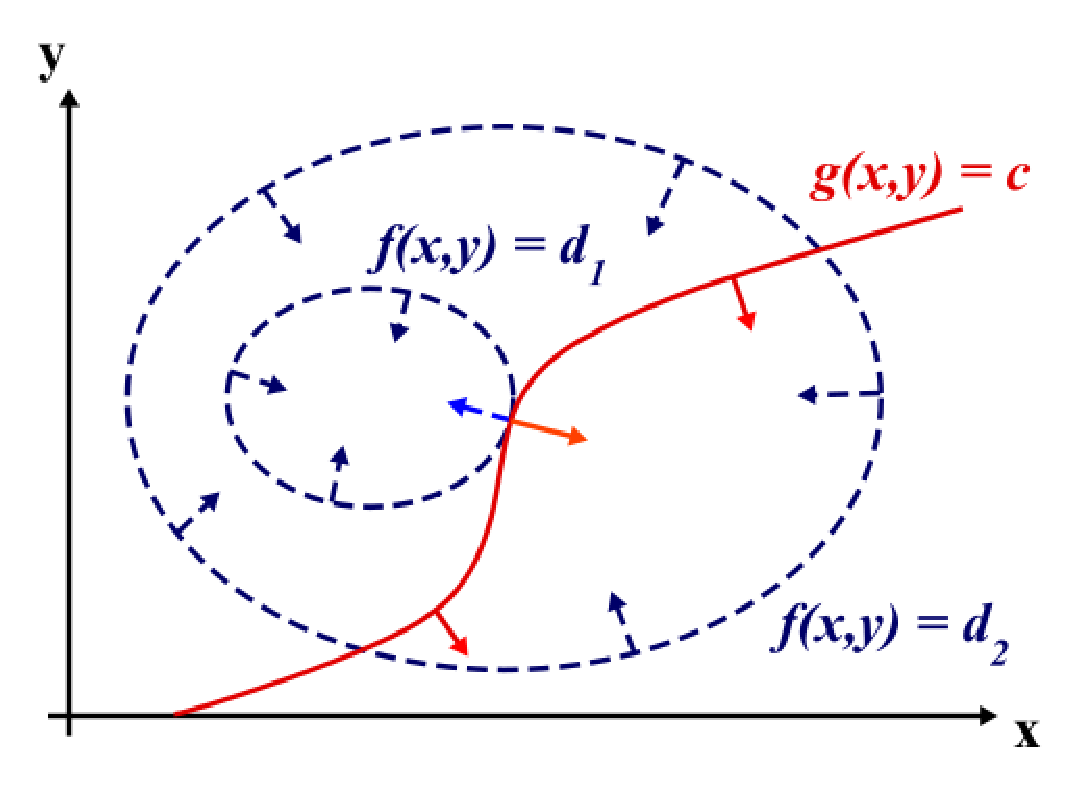
\epsfig{file=figures/lagrange_multipliers.eps,width=\textwidth}
\caption[Illustration of Lagrange multiplier method]
{\label{fig:LagrangeMultipliers} \textit{Illustration of Lagrange Multiplier
    Method (credit Wikipedia) showing two contour lines of the objective
    function $f(x,y) = d_i$ (dark blue dashed lines) and the nonlinear
    constraint $g(x,y)=c$ (red solid line) as well as their gradients (blue
    and red arrows) at various positions including the constrained optimum
    (light blue and orange arrows).}
}
\end{figure}

The general nonlinear programming problem can be solved mathematically using
Lagrange's method. It assumes that the constraints cannot be used to
explicitly reduce the parameter space of the iteration variables - as it is
typically the case for non-linear constraints and objective functions - and is
therefore a powerful method applicable to a general class of problems.

If we assume for simplicity that we have a 2D problem with only one equality
constraint $c(x,y) = 0$, we know that we only need to search for the optimum
along that constraint. At the optimum, the value of the objective function
will then be stationary, i.e. it does not locally increase or decrease along
the constraint. As the gradient of a function is perpedicular to its contour
lines of $f(x,y) =d$, this is equivalent to saying that the gradient of the
objective function at that point is parallel to the gradient of the
constraints:
\begin{equation}
\label{eqn:lagrangeequality}
\nabla f(x,y) = - \lambda \nabla c(x,y),
\end{equation}
where the factor $\lambda$ is necessary as only the direction, but not the
magnitude nor the sign of the gradients need to be equal. This is also
illustrated in Figure~\ref{fig:LagrangeMultipliers}.

When expanding the method to several equality and inequality constraints we
can make use of the {\it Lagrange function}. For the nonlinear programming
problem described by \ref{eqn:NPP} it is given by
\begin{equation}
L(\vec{x},\vec{\lambda}) = f(\vec{x}) - \sum_{i=1}^{m} \lambda_i c_i(\vec{x}),
\end{equation}
with the corresponding {\it Lagrangian multipliers} $\lambda_i$. It allows us
to formulate the {\it first order necessary} conditions for a constrained
optimum $\vec{x}^*$ with corresponding Lagrange multipliers $\vec{\lambda}^*$,
the Karush-Kuhn-Tucker (KKT) conditions,
\begin{subequations}
\begin{align}
\nabla_x L(\vec{x}^*,\vec{\lambda}^*)  &= \nabla_x f(\vec{x}^*) - \sum_{i=1}^{m} \lambda_i \nabla_x c_i(\vec{x}^*) = 0,&&\\
\label{eqn:compl}
\lambda^*_i c_i(\vec{x}^*)       &= 0,                                             &i&=1,\dots,m,\\
c_i(\vec{x}^*)                   &= 0,                                             &i&=1,\dots,k,\\
\lambda^*_i                &\geq 0,                                          &i&=k+1,\dots,m,\\
c_i(\vec{x}^*)                   &\geq 0,                                         &i&=k+1,\dots,m.
\end{align}
\label{eqn:KKT}
\end{subequations}
Please note that by construction the Lagrange multipliers $\lambda_i^*$
fulfilling the KKT conditions are describing the derivative of the objective
function with respect to the constraint equation $\frac{df}{dc_i}$ and are
therefore a measure of how much the objective function changes with respect to
each constraint.

In the special case of a {\it continuously differentiable convex} objective
function $f(\vec{x})$ and equality constraints as well as {\it affine}
inequality constraints, these KKT conditions are also sufficient for a global
optimum. The \process\/ optimisation solver has been designed to converge on
the KKT conditions, but does not test whether these are {\it sufficient} for a
global optimum. It is therefore crucial that the user verifies that a global
optimum has been found.

Furthermore, these conditions and therefore the solver, assume that both the
objective function and constraints are at least {\it first order continuously
  partially differential}, i.e. that their first order partial derivatives are
all continuous functions. This might not always be the case in \process\/ and
is a potential source of errors.

\section{Sequential Quadratic Programming (SQP)}
\label{sec:SQP}
Based on the Lagrange method, sequential (also successive or recursive)
quadratic programming is the most efficient method to numerically solve
constrained nonlinear optimisation problems \cite{Schittkowski1980}. It
combines a simple solver for a quadratic optimisation problem with linear
constraints that determines a search direction $\vec{\delta}$ with a line
search to find an optimum along that search direction. It is a type of the
more general {\it feasible direction} methods which is itself a type of {\it
  primal method} that solve nonlinear programming problems in the $n-m$
dimensional feasible subspace \cite{Luenberger2008}.

% flow diagram of VMCON

\begin{figure}
\begin{centering}
\begin{tikzpicture}[scale=0.88,transform shape]
 
  %%%%%%%%%%%%%%%%%%%%%%%%%%%%%%%
  % Draw diagram elements

  %setup
  \path \boxwsubs {1}{Setup}{initialise $\mat{B}$\item evaluate $f$, $\vec{c}$, $\nabla_x f$, $\nabla_x \vec{c}$ \item j=0, \texttt{nfev}=1};

  %beginning of j-Iteration
  \path (p1.south)+(0.0,-1.5) \boxes{2}{Solve QSP, $j=j+1$};
  \path (p2.south)+(0.0,-1.) \boxes{3}{calculate $\vec{\lambda}^j$, $\nabla_x L$, $\vec{\mu}^j$, l = 1};
  \path (p3.south)+(0.0,-1.) \boxes{4}{test convergence};
 
  % Line search
  \path (p4.south)+(0.0,-1.5) \boxes{5}{Evaluate $\Phi(f,\vec{c})$};
  \path (p5.south)+(2.5,-1.5) \boxwsubs{6}{l == 1}{calculate $\Delta$ \item set $\alpha=1$};
  \path (p5.south)+(-2.5,-3.0) \boxwsubs{7}{l $>=$ 1}{test convergence \item calculate $\alpha$};
  \path (p7.south)+(2.5,-1.75) \boxes{8}{update $\vec{x}^j$, evaluate $f$, $\vec{c}$, \texttt{nfev} += 1, l += 1};

  %end of j-Iteration
  \path (p8.south)+(0.0,-1.25) \boxes{9}{evaluate $f$, $\vec{c}$, $\nabla_x f$, $\nabla_x \vec{c}$, calculate $\nabla_x L$ };
  \path (p9.south)+(0.0,-1.0) \boxes{10}{BFGS update};

  %%%%%%%%%%%%%%%%%%%%%%%%%%%%%%%
  % Draw arrows between elements

  %setup
  \path [line] (p1.south) -- node [above] {} (p2);
  \exit{p1}{0}

  %beginning of j-Iteration
  \path [line] (p2.south) -- node [above] {} (p3);
  \exithigher{p2}{5}
  \exitlower{p2}{6}
  \path [line] (p3.south) -- node [above] {} (p4);
  \path [line] (p4.south) -- node [above] {} (p5);
  \exitsucc{p4}{1}

  %Line search
  \path [line] (p5.south) -- +(0.0,-0.25) -- +(+2.5,-0.25)
  -- node [above, midway] {} (p6);
  \exitright{p6}{4}
  \path [line] (p5.south) -- +(0.0,-0.25) -- +(-2.5,-0.25)
  -- node [above, midway] {} (p7);
  \exitleft{p7}{3}
  \path [line] (p7.west)  |- +(-1.,-0.25)
  |- node [above, midway] {} (p9.west);

  %fix
  \path [linepart] (p7.west)  |- +(-1.,0.25)
  |- node [right, pos=0.4] {adhoc fix} (p2.west);

  \path [line] (p6.south) -- +(0.0,-0.5) |- +(-2.5,-1.9)
  -- node [above, midway] {} (p8);
  \path [line] (p7.south) -- +(0.0,-0.25) -- +(+2.5,-0.25)
  -- node [above, midway] {} (p8);
  \exit{p8}{2}
  \path [line] (p8.west)  |- +(-2.75,0.0)
  |- node [above, midway] {} (p5.west);

   %end of j-Iteration
  \path [line] (p9.south) -- node [above] {} (p10);
  \path [line] (p10.west)  |- +(-4.0,0.0)
  |- node [above, midway] {} (p2.west);

  %%%%%%%%%%%%%%%%%%%%%%%%%%%%%%%
  % Draw background boxes
 
  \outerbackground{p7}{p2}{p6}{p10}{SQP iteration}
  \mybackground{p7}{p5}{p6}{p8}{Line search}
  
\end{tikzpicture}
\caption[Flowchart of the \vmcon\ optimisation solver] { \textit{This is the
    flow chart of the \vmcon\/ optimisation solver. The criteria for and the
    interpretation of the successful (\ifail\/ = 1) and unsuccessful (\ifail\/
    $\neq$ 1) return parameters are described in Table \ref{tab:ifail}. }
\label{fig:vmconflow}
}
\end{centering}
\end{figure}

%%%%%%%%%%%%%%%%%%%%%%%%%%%%%%%%%%%%%%%%%%%
% VMCON return parameters

\begin{table}
\footnotesize
\begin{center}
\begin{tabular}{|c|p{2.7cm}|p{3.4cm}|p{3.4cm}|}
  \hline
  \ifail\/ & Description & Meaning & Recommendation \\
  \hline
  \colorbox{red!20}{ 0 }&\vmcon: Improper input parameters & The input
  parameters to the solver are wrong, e.g. negative number of iteration
  variables. & This needs to be fixed on the developer side and should only
  occur in the test phase of new modules. \\
  \hline
  \colorbox{green!20}{ 1 } &\vmcon: Normal return & \vmcon\/ has found a
  solution that fulfills the necessary conditions within the specified error
  tolerances (c.f. eq. \ref{eqn:vmcon_errtol}). & Test whether the solution is
  a global solution by using different starting parameters.\\
  \hline
  \colorbox{red!20}{ 2 } & Too many function calls & During the line search
  \vmcon\/ has reached the maximum number of total function calls
  (\texttt{maxfev}=100)  & \vmcon\/ struggles to find a solution. Retry with
  different start parameters. \\
  \hline
  \colorbox{red!20}{ 3 } & Line search required 10 functions calls & The
  results produced by input objective function/constraints and  their
  gradients are inconsistent. This can be due to numerical noise in the input
  functions. & The developer needs to check the consistency and numerical
  robustness of the objective function, constraints and their
  derivatives. Perhaps the accurracy in numerical
  integrations/differentiations needs to be higher. As a user, try changing
  the iteration bounds or adding other iteration variables. \\
  \hline
  \colorbox{red!20}{ 4 } & Uphill search direction was calculated & The
  quadratic subproblem has suggested a search direction in which the objective
  function only increases.  & This happens if an inconsistency between the
  objective function, the constraints and their respective derivatives occurs
  (c.f. \ifail\/ =3).\\
  \hline
  \colorbox{red!20}{ 5 }&\texttt{qpsub}: No feasible solution or bad
  approximation of Hessian & Either no optimum lies within the space allowed
  by the constraints and variable bounds or the identity matrix is not a good
  first approximation of the Hessian. & As a user, add a new iteration
  variable, as developer, try using a multiple of the identity matrix as
  initial Hessian instead.\\
  \hline
  \colorbox{red!20}{ 6 } &\texttt{qpsub}: Singular matrix in quadratic
  subproblem or restriction by artificial bounds & This is fairly
  self-explanatory. & If this is meaningful, widen the boundaries of the
  iteration variables.  \\
  \hline
\end{tabular}
\end{center}
\caption{Summary of the description and  meaning of the \vmcon\/ return
  parameters \ifail\/. }
\label{tab:ifail}
\normalsize
\end{table}

\section{\vmcon}
\label{sec:vmcon}
The optimisation solver implemented in \process\/ is the Fortran routine
\vmcon\/ \cite{vmcon}. It is a modified version of the \texttt{vf02ad} routine
from the Harwell Software Library\footnote{www.hsl.rl.ac.uk} and implements a
SQP method originally suggested by Powell\footnote{This should not be confused
  with Powell's algorithm \cite{Powell1964} which solves a multidimensional
  unconstrained minimisation problem without derivatives.}~\cite{Powell1978}
based on work by Han \cite{Han1975}.  As stated before \vmcon\/ is designed to
converge on a solution of the {\it necessary} KKT conditions \ref{eqn:KKT}, but
does not check the {\it sufficient} conditions. Its convergence criterion is
therefore given by
\begin{equation}
\label{eqn:vmcon_errtol}
\left| \nabla_x f(\vec{x}^{j-1})^T \cdot \vec{\delta}^{j} \right| +
\sum^m_{i=1}\left| \lambda^j_i c_i(\vec{x}^{j-1}) \right| < \texttt{epsvmc}
\end{equation} %Yes, the j and j-1 are correct!
where \texttt{epsvmc} is a user specified error tolerance, $\vec{\delta}^j$ is
the vector in direction of the next line search (c.f. section
\ref{sec:linesearch}) and $j$ is the counter of the sequential quadratic
programming iteration. Hence, the first part estimates the predicted
improvement due to the next line search and the second part measures the error
in the complimentary condition \ref{eqn:compl} of the KKT conditions.

Figure \ref{fig:vmconflow} describes the flow chart of the \vmcon\/ routine,
while the various values of the return parameter \ifail\/\footnote{Note,
  within the \vmcon\/ routine \ifail\/ is called \texttt{info}.} are described
and interpreted in Table~\ref{tab:ifail}.

\section{The Quadratic Subproblem (QSP)}
\label{sec:QSP}
Within sequential quadratic programming the complex nonlinear problem is
broken down into solving a sequence of local quadratic subproblems with linear
constraints. This is based on the assumption that locally the problem is well
approximated by a second order Taylor expansion of the Lagrange
function. %Not the objective function!!!!
Hence, the local quadratic subproblem is described by
\begin{subequations}
\begin{align}
\textnormal{minimise } &Q(\vec{\delta}) = f(\vec{x}^{j-1}) + \vec{\delta}^T
\nabla_x f(\vec{x}^{j-1})+ \frac{1}{2} \vec{\delta}^T \nabla_{xx}
L(\vec{x}^{j-1},\vec{\lambda}^{j-1})\vec{\delta} \\
\textnormal{subject to } &\vec{\delta}^T \nabla_x c_i (\vec{x}^{j-1}) +
c_i(\vec{x}^{j-1}) = 0,\ i = 1,\dots,k,\\
\textnormal{and } &\vec{\delta}^T \nabla_x c_i (\vec{x}^{j-1}) +
c_i(\vec{x}^{j-1}) \geq 0,\ i = k+1,\dots,m,
\end{align}
\end{subequations}
where $\vec{\delta} = \vec{x} - \vec{x}^{j-1}$, the index $j-1$ indicates the
parameter values of the previous iteration\footnote{Note $j$ is called
  \texttt{nqp} in the \vmcon\/ routine.} and
$\nabla_{xx}L(\vec{x}^{j-1},\vec{\lambda}^{j-1})$ is the Hessian of the
Lagrange function. The solution of the QSP $\vec{\delta}$ describes the change
of the current iteration variable vector that minimises the local
approximation of the problem. To assure convergence even from bad starting
points, it is not directly used to update the iteration variable vector, but
describes the direction of the line search in which a 1d function is minimised
using a Newtonian method (c.f. section \ref{sec:linesearch}). Being a second
order approximation to the original problem, it typically has a faster
convergence that sequential linear programming (SLP) methods
\cite[chap. 10.4]{Bazaraa1993}.

To allow the applicability of the solver to more general problems, Powell
\cite{Powell1978} substituted the Hessian
$\nabla_{xx}L(\vec{x}^{j-1},\vec{\lambda}^{j-1})$ with a positive definite
approximation $\mat{B}$. This means that both the objective function
$f(\vec{x})$ and the constraint equations $c_i(\vec{x})$ only have to be
continuously differentiable instead of twice continuously differentiable with
respect to the iteration variable vector $\vec{x}$. This makes the method a
Quasi-Newtonian method as opposed to true Newtonian methods. How this
approximation is initialised and updated is described in more detail in the
section about the Broyden-Fletcher-Goldfarb-Shanno update \ref{sec:BFGS}.

To solve the QSP \vmcon\/ uses \texttt{harwqp} a modification of the the
Harwell library routine \texttt{VE02AD}, which in itself uses the subroutine
\texttt{harwfp/LA02AD} to find a feasible point within the variable bounds and
linearised constraints. Both routines go back to a method by Fletcher
\cite{Fletcher1970a,Fletcher1970b,Fletcher1970c}. The Lagrange multipliers are
also determined from results of the \texttt{harwqp} routine.

If the routine cannot find a feasible point it fails with \ifail\/ = 5
(c.f. Table \ref{tab:ifail}). As the routine is only checking the local linear
approximation of the constraints rather the full non-linear constraints, there
is a chance that a feasible point exists even though the routine fails with
\ifail\/ = 5. In these cases, it is possible that the first approximation of
the Hessian has not been good and the algorithm has, therefore, taken an
inappropriately large step. Then using a multiple of the identity matrix will
improve convergence of the algorithm.

If a singular matrix is encountered with the QSP solver or the solution is
restricted by the artificial bounds, \vmcon\/ fails with \ifail\/ = 6.  In
this case it can be helpful to widen the boundaries of the iteration
variables.



\section{The Line Search}
\label{sec:linesearch}

The line search is an essential part of the SQP algorithm. As Powell
\cite{Powell1978} pointed out, it is necessary to allow convergence from poor
starting conditions. It uses the vector $\vec{\delta}$ from the QSP to update
$\vec{x}^j = \vec{x}^{j-1} + \alpha^j \vec{\delta}^j$ where the step-length
parameter $\alpha^j>0$ is determined by the line search as the parameter that
minimises
\begin{equation}
\Phi(\alpha) = f(\vec{x}) + \sum_{i=1}^k \mu_i \left| c_i(\vec{x})\right| +
\sum_{i=k+1}^m \mu_i \left| min(0,c_i(\vec{x}))\right|
\end{equation}
where the weights are defined as
\begin{equation}
\mu_i = 
\begin{cases}
|\lambda_i^1| & \textnormal{ if } j = 1,\\
max\left(|\lambda_i^j|,1/2(\mu_i^{j-1} + |\lambda_i^j|)\right) & \textnormal{ if } j > 1
\end{cases}
\end{equation}
to assure maximally efficient convergence \cite{Han1975}. Note, that in this
method locally {\it inactive} inequality constraints (see Userguide)
are not having any effect. It should always be possible, to find a solution
that fulfills
\begin{equation}
\Phi(\alpha=0)> \Phi(\alpha^j),
\end{equation}
if 
\begin{equation}
\left. \frac{d \Phi}{d\alpha}\right|_{\alpha=0} < 0.
\end{equation}
In case the derivative is positive (\texttt{dflsa} $\geq 0$), an uphill search
direction has been determined and the code stops with \ifail\/ =
4. %XXX(Though I don't think this dflsa is actually the true derivative!)
This typically only happens, if the objective function or constraints are
inconsistent with their own derivatives.

As the line search tries to determine the optimum of a one dimensional, but
fully non-linear function $\Phi(\alpha)$, it creates a series of $\alpha_l$
values\footnote{In the actual code $\alpha=$\texttt{calpha} and $\alpha_l
  =$\texttt{alpha}$*\alpha_{l-1}$.}. At each iteration $l$, a quadratic local
function $\Phi_l(\alpha)$ fullfilling the boundary conditions $\Phi_l(0) =
\Phi(0)$, $\Phi_l'(0)=\Delta$ and $\Phi_l(\alpha_{l-1}) = \Phi(\alpha_{l-1})$
is minimised, where typically
$\Delta=\Phi'(0)$. %XXX But I don't think this is the case in \vmcon (see comment above).
This leads to
\begin{equation}
\Phi_l(\alpha) = \Phi(0) + \Delta \alpha + \frac{\Phi(\alpha_{l-1})-\Phi(0) -
  \Delta \alpha_{l-1}}{\alpha_{l-1}^2} \alpha^2
\end{equation}
and minimising this gives 
\begin{equation}
\alpha_{min} = - \frac{\Delta\alpha_{l-1}^2}{2(\Phi(\alpha_{l-1})-\Phi(0) -
  \Delta \alpha_{l-1})}.
\end{equation}
Powell then sets $\alpha_l = \min(\alpha_{min}, 0.1\alpha_{l-1})$. On each
iteration the convergence of the line search is tested. It is reached, if
\begin{equation}
\Phi(\alpha_l) - \Phi(0) < 0.1 \Delta.
\end{equation}
which assures that the change in the function is small in comparison to its
derivative and 0.1 is a factor determined by experience. If this criterion is
successful, the code exits the line search and updates all function
evaluations.

As a modification to the original code, we have added an adhoc fix that exits
the line search in the case of
\begin{equation}
\Phi(\alpha_l) - \Phi(0) > 0.
\end{equation}
This has been added as experience have shown that \vmcon\/ typically does not
converge in these situations, but if it is forced to caculate a new search
direction in this way, it sometimes successfully finishes. Note, that this
cannot force \vmcon\/ to converge on any false solutions, as it only exits
positively when the convergence criterion \ref{eqn:vmcon_errtol} is fulfilled.

Typically, the line search already converges after one iteration and,
therefore, $\alpha = 1$. Hence, the \vmcon\/ line search has an upper limit of
maximally 10 iterations before it terminating with \ifail\/ = 3 (c.f. Table
\ref{tab:ifail}). This is higher than Powell's original limit of 5 to avoid a
few cases of early termination without a major effect on efficiency.

Within the line search \vmcon\/ also checks that the total number of function
calls has not exceeded \texttt{maxfev} = 100. If this is the case, it exits
with error code \ifail\/ = 2. Both checks assure that the routine stops, if it
does not seem to be able to find a solution.


\section{The Broyden-Fletcher-Goldfarb-Shanno (BFGS) quasi-Newton update}
\label{sec:BFGS}

\vmcon\/ uses a quasi-Newtonian update, the Broyden-Fletcher-Goldfarb-Shanno
update, in the approximation of the Hessian of the Lagrange function. This
means it is applicable to all continuously differentiable objective and
constraint functions. Note, that due to the constraints it is not actually
necessary for the Hessian of the solution to be positive definite, even though
this is essential for the convergence of the algorithm.

In quasi-Newtonian methods the identity matrix $\mat{I}$ is often chosen as an
initial estimate of the Hessian because of its positive definiteness. In some
cases it can be helpful to chose a constant multiple of the identity matrix
instead. The BGFS update \cite{Avriel2003} is one way of revising the initial
Hessian approximation using the update of the iteration variable vector
\begin{equation}
\vec{\xi} = \vec{x}^{j} - \vec{x}^{j-1}
\end{equation}
and the update of the Jacobian of the Lagrange function
\begin{equation}
\vec{\gamma} = \nabla_x L(\vec{x}^j,\vec{\lambda}^{j}) - \nabla_x
L(\vec{x}^{j-1},\vec{\lambda}^{j}). %NOT \lambda^{j-1}!!!
\end{equation}
Note that unless $\alpha=1$ in the line search, $\vec{\xi} \neq
\vec{\delta}$. To assure the positive definiteness of $\mat{B}$ Powell
\cite{Powell1978} suggested a variation of the standard formalism that uses
$\vec{\eta}$ instead of $\vec{\gamma}$
\begin{equation}
\vec{\eta} = \theta \vec{\gamma} + (1-\theta) \mat{B} \vec{\xi}
\end{equation}
with 
\begin{equation}
\theta = \left\{
\begin{array}{lr}
1 & \vec{\xi}^T \vec{\gamma} \geq 0.2 \vec{\xi}^T \mat{B} \vec{\xi} \\
\frac{0.8 \vec{\xi}^T B \vec{\xi}}{\vec{\xi}^T} & \vec{\xi}^T \vec{\gamma} <
0.2 \vec{\xi}^T \mat{B} \vec{\xi}
\end{array}
\right.
\end{equation}
to calculate a new approximation of the Hessian
\begin{equation}
\mat{B}_{new} = \mat{B} - \frac{\mat{B} \vec{\xi} \vec{\xi}^T
  \mat{B}}{\vec{\xi}^T \mat{B} \vec{\xi}}+\frac{\vec{\eta}^T
  \vec{\eta}}{\vec{\xi}^T \vec{\eta}}.
\end{equation}
Using the modified version of the BFGS update as suggested by Powell,
furthermore, assures superlinear convergence, even if the true Hessian is
indefinite \cite{Powell1977}.

\section{Symbols}
\label{sec:symbols}
In the previous sections the following conventions have been assumed:
$\vec{x}$, $\vec{\delta}$, $\vec{\xi}$, $\vec{\gamma}$ and $\vec{\eta}$ are
$n$-dimensional vectors, where $n$ is the number of iteration
variables. $\vec{c}$, $\vec{\lambda}$, $\vec{\mu}$ are $m$-dimensional
vectors, where $m$ is the total number of constraints and $c_i$, $\lambda_i$
and $\mu_i$ ($i=1\dots m$) are their respective components. $\mat{B}$ and
$\mat{I}$ are $n\times n$-dimensional matrices, while $\nabla_x \vec{c}$ is an
$n\times m$-dimensional matrix.

\bibliographystyle{unsrt}
\bibliography{optsolverdoc}



\end{document}
